\documentclass[letterpaper, 10pt, journal]{IEEEtran}
\usepackage{graphicx}
\usepackage{float}
\usepackage{listings}
\usepackage{color}
\usepackage{multirow}
\usepackage[table,xcdraw]{xcolor}
\usepackage[justification=centering]{caption}
% Paquete para referenciar figuras
\usepackage{nameref}
\graphicspath{ {./Images/} }
% Paquetes para las funciones matematicas
\usepackage{amsmath}
\usepackage{amssymb}

\usepackage[justification=centering]{caption}
\lstset{frame=tb,
  language=Java,
  aboveskip=3mm,
  belowskip=3mm,
  showstringspaces=false,
  columns=flexible,
  basicstyle={\small\ttfamily},
  numbers=none,
  numberstyle=\tiny\color{gray},
  keywordstyle=\color{blue},
  commentstyle=\color{dkgreen},
  stringstyle=\color{mauve},
  breaklines=true,
  breakatwhitespace=true,
  tabsize=3
}

\begin{document}
\title{Tarea 1 - Reporte de \LaTeX  }
\author{Kathy~Brenes~Guerrero, Barnum~Castillo~Barquero

~\IEEEmembership{
    \begin{center}
        Maestr\'ia en Ciencias de la Computaci\'on, Introducci\'on a la Investigaci\'on, ITCR
    \end{center}
}}% <-this % stops a space

% The paper headers
\markboth{Instituto Tecnol\'ogico de Costa Rica, Introducci\'on a la Investigaci\'on, Agosto~2018}%
{Shell \MakeLowercase{\textit{et al.}}: Tarea 1 - Reporte de \LaTeX  }
\maketitle

\begin{abstract}
One of the biggest issues that an operating system can experience is privilege escalation. Privilege escalation is the act of exploiting a bug, design flaw, or configuration oversight in an operating system or software application to gain elevated access to resources that are normally protected from an application or user. Understanding the weaknesses and flaws of a security level issue for the operating system can help implement better approaches and techniques to improve the software itself. Just because you have updated your computer to the latest update or patch, doesn’t mean that it has been secured. Windows, for example, has a series of vulnerabilities that can affect the operating system and can't be solved by Microsoft because the updates can create incompatibilities with an older system or with some security protocols. The Privilege Escalation technique takes advantage of these vulnerabilities to  gain privileges (access) within a remote  system, in order to run applications and make commands on it. The focus of this paper is to list the vulnerabilities that have been demonstrated by third party systems in different operating system, and provide a technical point of view  on what can be done to avoid these breaches ( vulnerabilities or impacts). An Operation System breach can enable attackers to increase their level of control over target systems, such that they are free to access any data or make any configuration changes. This study reveals the importance of the way in which current systems should be defended from this mechanism.
\end{abstract}
\begin{IEEEkeywords}
Operating System, Penetration Testing, Cybersecurity, Internet of Things.
\end{IEEEkeywords}

\section{Introducci\'on}
El siguiente reporte detalla los conceptos b\'asicos y principales del lenguaje de programaci\'on LaTeX, adem\'as de su historia. Cada una de las siguientes secciones incorpora un ejemplo aplicado de los t\'erminos comentados.
\section{Historia de \LaTeX  }
TeX es el programa original de composici\'on matem\'atica desarrollado alrededor de 1980 por Donald Knuth  para la composici\'on tipogr\'afica digital de alta calidad.\cite{[3]} TEX es un lenguaje de bajo nivel con el que las computadoras pueden trabajar, pero a la mayor\'ia de las personas les resultar\'ia dif\'icil usarlo; entonces \LaTeX   ha sido desarrollado para hacerlo m\'as f\'acil.\cite{[2]}.Se pronuncia como "tecnolog\'ia" como en alta tecnolog\'ia. La X es la letra griega chi, que hace que el sonido "ch" aparezca al final de "tech". En la documentaci\'on original para TeX, hay mucha discusi\'on acerca de "pegar" objetos juntos y de "estirar" el espacio entre los objetos que componen una p\'agina. \cite{[3]}

El l\'{a}tex es un producto natural pegajoso que forma la base del caucho, y creo que ese es el motivo de la palabra LaTeX. LaTeX est\'{a} construido sobre TeX. Fue escrito a principios de la d\'{e}cada de 1980 por Leslie Lamport. Tiene m\'{a}s funciones de alto nivel integradas que TeX, por lo que tiende a ser m\'{a}s f\'{a}cil de usar. LaTeX no es un intento de sonar en franc\'{e}s; probablemente no sea La TeX, o "The TeX". La raz\'{o}n de la divertida alternancia de letras may\'{u}sculas y min\'{u}sculas es que TeX y LaTeX, cuando se escriben correctamente de esta manera:, son todas letras may\'{u}sculas pero en diferentes tama\~{n}os de puntos y diferentes alturas por encima y por debajo de la l\'{\i}nea de base. Alternando may\'{u}sculas y min\'{u}sculas imita esto. \cite{[3]}
\newline
\LaTeX   se cre\'o para facilitar la producci\'on de libros y art\'iculos de uso general dentro de TeX. Debido a que \LaTeX   es una extensi\'on del sistema de composici\'on tipogr\'afica TeX, tiene la capacidad de TeX para compilar documentos t\'ecnicos que contienen ecuaciones matem\'aticas complejas. Esta caracter\'istica hizo que LaTeX fuera popular entre cient\'ificos e ingenieros. \cite{[1]}
\newline
La producci\'on de un documento \LaTeX   comienza con un archivo de texto que contiene contenido etiquetado con c\'odigos especiales \LaTeX   utilizados para indicar c\'omo se dise\~nar\'a el texto. Cuando el archivo se ejecuta a trav\'es de un procesador \LaTeX  , se producen p\'aginas de composici\'on tipogr\'afica. Debido a que la composici\'on tipogr\'afica \LaTeX   requiere envolver el texto en c\'odigos inform\'aticos complicados, tiene una curva de aprendizaje bastante empinada. Aunque ahora hay programas de software que ayudan a automatizar la creaci\'on de documentos \LaTeX  , un conocimiento pr\'actico de \LaTeX   sigue siendo deseable para este tipo de composici\'on tipogr\'afica.
\newline
\LaTeX   fue uno de los primeros programas de composici\'on tipogr\'afica capaz de producir ecuaciones matem\'aticas complejas. Con los a\~nos se ha utilizado para componer muchas revistas cient\'ificas, matem\'aticas y de ingenier\'ia. La American Mathematical Society (AMS) incluso tiene su propio conjunto de extensiones, llamado AMS-LaTeX, que sus contribuyentes usan para su revista. Pero los programas de autoedici\'on como Quark Inc. de Quark Inc. y FrameMaker de Adobe Systems Incorporated se volvieron m\'as capaces de producir expresiones matem\'aticas complejas, \LaTeX   se hizo menos popular.\cite{[1]}
La versi\'on actual de \LaTeX   es \LaTeX 2e. \cite{[2]}


\section{Usos acad\'emicos, extensi\'on, importancia}
\LaTeX    es un sistema de preparaci\'on de documentos para producir documentos de aspecto profesional, no es un procesador de textos. Es particularmente adecuado para producir documentos largos y estructurados, y es muy bueno para escribir ecuaciones. Est\'a disponible como software libre para la mayor\'ia de los sistemas operativos.
\newline
Si est\'a acostumbrado a producir documentos con Microsoft Word, encontrar\'a que \LaTeX   es un estilo de trabajo muy diferente. Microsoft Word es \''Lo que ves es lo que obtienes\'' (WYSIWYG), esto significa que puedes ver c\'omo se ver\'a el documento final mientras escribes. Cuando trabaje de esta manera, probablemente realice cambios en la apariencia del documento (como espacios entre l\'ineas, encabezados, saltos de p\'agina) mientras escribe. Con \LaTeX   no ver\'a c\'omo se ver\'a el documento final mientras lo est\'a escribiendo; esto le permite concentrarse en el contenido m\'as all\'a de la apariencia.
Para producir esto en la mayor\'ia de los sistemas de tipograf\'ia o procesamiento de textos, el autor deber\'ia decidir qu\'e dise\~no usar, por lo que seleccionar\'ia (digamos) 18pt Times Roman para el t\'itulo, 12pt Times Italic para el nombre, y as\'i sucesivamente. Esto tiene dos resultados: los autores pierden su tiempo con los dise\~nos; y muchos documentos mal dise\~nados. \cite{[2]}
LaTeX se basa en la idea de que es mejor dejar el diseño del documento a los diseñadores de documentos y permitir que los autores continúen con la escritura de documentos. \cite{[2]}
\newline
Un documento \LaTeX   es un archivo de texto sin formato con una extensi\'on de archivo .tex. Se puede escribir en un editor de texto simple como el Bloc de notas, pero la mayor\'ia de las personas encuentran que es m\'as f\'acil usar un editor de \LaTeX   dedicado. Mientras escribe, marque la estructura del documento (t\'itulo, cap\'itulos, subt\'itulos, listas, etc.) con etiquetas. Cuando finaliza el documento, comp\'ilelo; esto significa convertirlo a otro formato. \cite{[2]}
\newline
Existen varios formatos de salida diferentes, pero probablemente el m\'as \'util sea Portable Document Format (PDF), que aparece tal como se imprimir\'a y se puede transferir f\'acilmente entre computadoras. \cite{[2]}
\newline
\textbf{Implementaciones de \LaTeX}
\begin{enumerate}
    \item Composici\'on de art\'iculos de revistas, informes t\'ecnicos, libros y presentaciones de diapositivas.
    \item Control sobre documentos grandes que contienen secciones, referencias cruzadas, tablas y figuras.
    \item Composici\'on tipogr\'afica de f\'ormulas matem\'aticas complejas.
    \item Composici\'on tipogr\'afica avanzada de las matem\'aticas con AMS-LaTeX.
    \item Generaci\'on autom\'atica de bibliograf\'ias e \'indices.
    \item Composici\'on tipogr\'afica multiling\"ue.
    \item Inclusi\'on de obras de arte, y color de proceso o mancha.
    \item Utilizando fuentes PostScript o Metafont.
\end{enumerate}

\subsection{Tipo de archivo}
Los archivos LaTeX no son tan self-contained como, por ejemplo, los documentos de Word. Sin embargo, sus tama\~{n}os de archivo son generalmente m\'{a}s peque\~{n}os. Aqu\'{\i} hay una descripci\'{o}n muy b\'{a}sica.
\newline
Un archivo fuente LaTeX debe recibir la extensi\'{o}n .tex. Es un archivo de texto, uno que puede editar con Notepad o SimpleText, a diferencia de los documentos de Word, que solo puede editar con Word. El archivo fuente LaTeX contiene el texto de sus documentos m\'{a}s los comandos que indican c\'{o}mo deben formatearse el texto y las ecuaciones. De esta manera, es un poco como c\'{o}digo de computadora o HTML sin formato.
\newline
Los archivos fuente LaTeX deben ser procesados por un programa que sepa c\'{o}mo interpretar los diversos comandos integrados en ellos. En una PC, puede descargar varias implementaciones de LaTeX, como MiKTeX. En Macintosh, puede usar OzTeX. En una m\'{a}quina UNIX, deber\'{\i}a ser capaz de instalar l\'{a}tex. Me referir\'{e} gen\'{e}ricamente a estos programas como l\'{a}tex. Tenga en cuenta que el programa texify puede ser el programa real que se utiliza para procesar un documento.
\newline
Cuando latex procesa un archivo fuente LaTeX llamado example.tex, crea un archivo llamado example.dvi. dvi significa DeVice Independent. Es un formato anterior a .pdf, y pretend\'{\i}a ser lo que dice, un formato que pueden manejar muchos dispositivos diferentes (plataformas de computadora). Cada plataforma de computadora tiene sus propios programas que pueden ver (algunos dicen vista previa) archivos .dvi. En una PC, MikTex viene con YAP (Yet Another Previewer), en Macintosh, una vista previa dvi est\'{a} integrada en OzTeX, y en una m\'{a}quina UNIX, generalmente puede encontrar un programa llamado xdvi. latex tambi\'{e}n produce un archivo .aux y .log, del cual no tenemos que preocuparnos ahora.
\newline
La progresi\'on habitual al componer un documento en LaTeX es escribir el archivo .tex usando un editor de texto, luego procesarlo usando latex, luego ver el resultado de .dvi usando un reproductor de vista previa. Comparado con Word, esto parece bastante torpe, lo s\'e. Se debe principalmente al hecho de que LaTeX se desarroll\'o en una plataforma UNIX, y as\'i es como los programas UNIX tienden a estructurarse. Porque Es m\'as modular y m\'as f\'acil tener a muchas personas involucradas en el desarrollo, en lugar de una sola empresa monol\'itica de desarrollo de software. En balance, eso es algo bueno.
\newline
No puede enviar un archivo .dvi a una impresora. La mayor\'{\i}a de las impresoras aceptan entradas PostScript (.ps). En una PC, puede abrir el archivo .dvi con YAP para imprimirlo. Con OzTeX, puede seleccionar Archivo, Imprimir. En UNIX, primero utiliza un programa como dvips para convertir el archivo .dvi a un archivo .ps, luego env\'{\i}a el archivo .ps a la impresora usando un comando como lp file.ps.
\newline
Finalmente, una vez que crea un documento LaTeX, puede compartir el resultado electr\'{o}nicamente con otros, ya sea por correo electr\'{o}nico como un archivo adjunto o por publicarlo en una p\'{a}gina web. Las personas que no usan TeX o LaTeX generalmente no tienen instaladas las previsualizaciones .dvi y .ps, pero a menudo tienen Adobe Acrobat Reader, que puede leer y visualizar archivos .pdf (Portable Document Format). En una PC, probablemente use pdflatex para procesar el c\'{o}digo fuente de LaTeX y producir salida .pdf autom\'{a}ticamente. O puede usar un convertidor de DVI a PDF como dvipdfm, que viene con MiKTeX. 
En un Macintosh, puede usar Adobe Distiller (use Sherlock para buscarlo, luego ejec\'{u}telo) para convertir un archivo .ps en un archivo .pdf, luego use Acrobat Reader para verlo. En UNIX, puede usar dvipdf o ps2pdf. La principal desventaja de producir directamente salida .pdf de l\'{a}tex al editar su archivo fuente .tex es que una vez que Adobe Reader tiene un archivo abierto, latex no puede modificar el archivo en el disco. Las previsualizaciones dvi como YAP no tienen este problema.

\section{Estilos de documento }
\begin{lstlisting}
    \documentclass[options]{article}
    Preamble (for LaTeX commands only)
    \begin{document}
    Document text (text with embedded LaTeX commands)
    \end{document}
\end{lstlisting}
Mediante el comando \textbf{document class} se determina el dise\~{n}o y la estructura general del documento. Adem\'{a}s la opci\'on \textbf{article} permite establecer espec\'ificamente los usos y las propiedades que se van a desarrollar, otras clases com\'{u}nmente utilizadas son:
\newline
\subsection{Article:} como su nombre indica, destinada a escribir art\'{\i}culos. Esto significa documentos relativamente cortos que no contienen cap\'{\i}tulos o partes, solo secciones, subsecciones, etc. Como una de las clases base, el formato es bastante b\'{a}sico. Sin embargo, como la clase de art\'{\i}culo proporciona la funci\'{o}n b\'{a}sica que la mayor\'{\i}a de la gente espera de LaTeX, a menudo se usa con modificaciones para documentos m\'{a}s largos.

\begin{lstlisting}
    \documentclass[opciones]{article}
    Preambulo (declaraciones : paquetes, comandos; título, autor, fecha)
    \begin{document}   Documento
    \maketitle
    \begin{abstract} ...
    \end{abstract}
    \section{... }
    \subsection{... }
    \subsubsection{...}
    \end{document}
\end{lstlisting}

\textbf{Comandos importantes}
\begin{enumerate}
\item \textbackslash maketitle Hace que se produzcan las lineas para el titulo, autor y fecha. Debe ubicarse despues de \textbackslash begin{document}, si se omite, no se generan dichos campos.
\item \textbackslash date Se imprime la fecha vigente del computador, o el valor que se ingrese al campo obligatorio, si se desea que no aparezca de debe escribir \textbackslash date{}.
\item \textbackslash thanks\{...\} Se puede utilizar en \textbackslash title, \textbackslash author, \textbackslash date,produce notas al pie de página con la informacion del autor.
\item \textbackslash begin\{abstract\}...\textbackslash end\{abstract\} En este entorno se coloca el resumen del articulo y debe ubicarse despues de \textbackslash maketitle.
\item \textbackslash section, \textbackslash subsection Son numeradas automaticamente.
\end{enumerate}

\subsection{Report:} La clase de informe est\'{a} destinada a documentos m\'{a}s largos que tendr\'{a}n cap\'{\i}tulos, mientras que el libro est\'{a} destinado a documentos muy grandes. La configuraci\'{o}n est\'{a}ndar para informe y libro es ligeramente diferente de art\'{\i}culo. Por ejemplo, el valor predeterminado para el art\'{\i}culo es poner la informaci\'{o}n de \textbackslash{} maketitle en la parte superior de la primera p\'{a}gina, mientras que el informe y el libro usan p\'{a}ginas de t\'{\i}tulo separadas. libro incluye accesos directos predefinidos para \textbackslash{} frontmatter (cap\'{\i}tulos sin numerar con n\'{u}meros de p\'{a}gina romanos), \textbackslash mainmatter (cap\'{\i}tulos numerados y n\'{u}meros de p\'{a}gina ar\'{a}bica) y \textbackslash backmatter.
Tiene la misma estructura de book. Imprime por una sola cara: \textbackslash oneside. El entorno abstract esta disponible, se crea en una p\'agina independiente.
\subsection{Thesis:} Para escribir una tesis de RPI.
\subsection{Book:} Para la estructura, formato y composici\'on de libros.
\begin{lstlisting}
\documentclass{book}
Preámbulo (declaraciones : paquetes, comandos; titulo, autor, fecha)
\begin{document}
\maketitle
\frontmatter
\mainmatter
\chapter{...}
\section{...}
\subsection{...}
\appendix
\backmatter
\end{document}
\end{lstlisting}

\textbf{Comandos importantes}
\begin{enumerate}
\item \textbackslash frontmatter :Apertura del libro, se presenta todo aquel contenido que no tenga que ver con el tema central tratado en el libro: pr\'ologo, agradecimientos, tabla de contenido, derechos de autor, \'indice de figuras, \'indice de tablas etc. La numeraci\'on se realiza utilizando numeraci\'on romana.
\item \textbackslash mainmatter Contiene la parte central del documento, se desarrolla el tema tratado en el libro, también se ubican los apéndices mediante el comando \textbackslash appendix los cuales se numeran con las letras mayusculas A, B, C,...
\item \textbackslash backmatter Es el cierre del documento, contiene el \'indice alfab\'etico, bibliograf\'ia, conclusiones, reconocimientos, informaci\'on editorial, etc. Los cap\'itulos no son numerados
\end {enumerate}

\subsection{Letter:} Para redactar el formato de una carta.
\begin{lstlisting}
\documentclass{letter}
\usepackage[spanish]{babel}
\usepackage[latin1]{inputenc}
\begin{document}
\address{
Revista Colombiana de Estadística \\
Universidad Nacional de Colombia}
\signature{
Pepito Pérez \\
Editor}
\date{30 septiembre de 2006}
\begin{letter}{
Dr. Donald Knuth \\
Departamento de Ciencias de la Computación \\
Universidad de Stanford \\
EEUU
}
\end{lstlisting}


\subsection{Slides:} Para el dise\~no y confecci\'on de las diapositivas elaboradas con Beamer.
El entorno slides da lugar a una transparencia, la numeraci\'on es consecutiva en la parte inferior derecha.
Slides no se utilizan \textbackslash chapter, \textbackslash section,
\textbackslash pagestyle, \textbackslash thispagestyle, ni los entornos table y figure. Los dem\'as comandos se pueden utilizar libremente.
\begin{lstlisting}
\documentclass{slides}
Preámbulo (declaraciones : paquetes, comandos; título, autor, fecha)
\begin{document}
\begin{slides}
Contenido de la transparencia
\end{slides}
\end{document}
\end{lstlisting}

Entre otras cosas, las clases proporcionan comandos de encabezado, como
\textbackslash{} part, \textbackslash{} chapter, \textbackslash{} section

\begin{lstlisting}
\documentclass[options]{article}
Preamble (for LaTeX commands only)
\begin{document}
Document text (text with embedded LaTeX commands)
\end{document}
\end{lstlisting}
\section{Uso de elementos}
\subsection{P\'arrafos}
Text here..
\subsection{Efectos de letra}
Text here..
\subsection{Tildes}
Text here..
\subsection{T\'itulos}
Text here..
\subsection{Subt\'itulos}
Text here..
\subsection{Referencias}
Text here..
\subsection{Marcas de agua}
Text here..
\subsection{Headers y Footers}
Text here..
\subsection{ Manejo de saltos de p\'agina}
Text here..
\subsection{Columnas de la p\'agina}
Text here..


\section{Manejo de Tablas}
Durante esta secci\'{o}n se estar\'{a}n discutiendo el atributo de Latex de creaci\'{o}n de tablas, partiendo del ejemplo de \textquotedblleft{}Tabla b\'{a}sica\textquotedblright{} incluyendo su c\'{o}digo en Latex hasta las diferentes caracter\'{\i}sticas para personalizarla seg\'{u}n las necesidades.

\subsection{Tabla B\'asica}
La siguiente tabla refleja la implementaci\'{o}n m\'{a}s b\'{a}sica, por razones de claridad se le ha agregado las l\'{\i}neas negras.

\begin{table}[H]\centering
\begin{tabular}{|l c|r|}
\hline
Columna 1 & Columna 2 & Columna 3 \\ \hline
Fila 11   & Fila 12   & Fila 13   \\ \hline
Fila 21   & Fila 22   & Fila 23   \\ \hline
\end{tabular}
\end{table}

El c\'{o}digo de la tabla es el siguiente:

\lstset{language=Java}
\begin{lstlisting}
\begin{table}[H]\centering
\begin{tabular}{|l c|r|}
\hline
Columna 1 & Columna 2 & Columna 3 \\ \hline
Fila 11   & Fila 12   & Fila 13   \\ \hline
Fila 21   & Fila 22   & Fila 23   \\ \hline
\end{tabular}
\end{table}
\end{lstlisting}

El comienzo de la tabla se representa con \textbackslash begin\textbackslash\{tabular\}, dentro de esta secci\'{o}n se describe el contenido de la tabla (Columna 1, Columna 2, etc), la separaci\'{o}n de la columna se da por \& y el de cada fila por \textbackslash\textbackslash. 

La alineaci\'on del texto se da por \{\textbar l\textbar c\textbar r\textbar\} siendo l = left, c = center, r = right y los s\'{\i}mbolos pipe (\textquotedblleft{}\textbar{}\textquotedblright{}) representa el delineado de las columnas, para delinear las l\'ineas horizontales se hace uso del \textbackslash{}hline al final de cada fila.

\subsection{Agregar columnas y filas}

Tomando el ejemplo de tabla b\'asica y agreg\'andole una nueva columna y una nueva fila da como resultado el siguiente c\'odigo.

\lstset{language=Java}
\begin{lstlisting}
\begin{table}[H]\centering
\begin{tabular}{|l|l|l|l|}
\hline
Columna 1  & Columna 2 & Columna 3 & C.Nueva \\ \hline
Fila 11    & Fila 12   & Fila 13   & \\ \hline
Fila 21    & Fila 22   & Fila 23   & \\ \hline
Nueva fila &           &           & \\ \hline
\end{tabular}
\end{table}
\end{lstlisting}

Las diferencias notorias como resultado de agregar la nueva fila y columna son \textquotedblleft{}Nueva fila \& \& \& \& \textbackslash{}\textbackslash{}hline\textquotedblright{} al final del c\'{o}digo que representa a la fila y en todas las columnas se ha agregado un \& dando la siguiente tabla.

\begin{table}[H]\centering
\begin{tabular}{|l|l|l|l|}
\hline
Columna 1  & Columna 2 & Columna 3 & C.Nueva \\ \hline
Fila 11    & Fila 12   & Fila 13   & \\ \hline
Fila 21    & Fila 22   & Fila 23   & \\ \hline
Nueva fila &           &           & \\ \hline
\end{tabular}
\end{table}

\subsection{M\'utiples columnas}
Para el proceso de combinar columnas en una misma fila es necesario el comando:

\lstset{language=Java}
\begin{lstlisting}
\multicolumn{ancho}{alineamiento}{contenido}
\end{lstlisting}

Teniendo en cuenta la l\'{\i}nea anterior y si lo agregamos al c\'{o}digo de tabla b\'{a}sica resulta en:

\begin{table}[H]\centering
\begin{tabular}{|l|l|l|}
\hline
Columna 1 & Columna 2  & Columna 3 \\ \hline
\multicolumn{2}{|l|}{Fila 11 + fila 12} & Fila 13 \\ \hline
Fila 21   & Fila 22    & Fila 23   \\ \hline
\end{tabular}
\end{table}

Conociendo la funci\'{o}n del comando multicolumn, podemos ver el c\'{o}digo agregado al de tabla b\'{a}sica y explicar su funcionamiento.

\lstset{language=Java}
\begin{lstlisting}
\begin{table}[H]\centering
\begin{tabular}{|l|l|l|}
\hline
Columna 1 & Columna 2 & Columna 3 \\ \hline
\multicolumn{2}{|l|}{Fila 11 + fila 12} & Fila 13 \\ \hline
Fila 21   & Fila 22   & Fila 23   \\ \hline
\end{tabular}
\end{table}
\end{lstlisting}

\{2\} es la cantidad de columnas que se expandi\'{o} la celda, \{\textbar{}l\textbar{}\} es la delineaci\'{o}n vertical de la celda m\'{a}s la alineaci\'{o}n del texto y el \'{u}ltimo par\'{a}metro es el contenido \textquotedblleft{}Fila 11 + fila12\textquotedblright{}.

\subsection{M\'utiples filas}
La funcionalidad de combinar filas es dada por el paquete.

\lstset{language=Java}
\begin{lstlisting}
\usepackage{multirow}
\end{lstlisting}

La siguiente tabla ejemplifica su uso.

\begin{table}[H]\centering
\begin{tabular}{|l|l|l|}
\hline
Columna 1                & Columna 2 & Columna 3 \\ \hline
\multirow{2}{*}{Fila 11 + fila 21} & Fila 12   & Fila 13   \\ \cline{2-3} 
                         & Fila 22   & Fila 23   \\ \hline
\end{tabular}
\end{table}

\lstset{language=Java}
\begin{lstlisting}
\begin{table}[H]\centering
\begin{tabular}{|l|l|l|}
\hline
Columna 1                & Columna 2 & Columna 3 \\ \hline
\multirow{2}{*}{Fila 11 + fila 21} & Fila 12   & Fila 13   \\ \cline{2-3} 
                         & Fila 22   & Fila 23   \\ \hline
\end{tabular}
\end{table}
\end{lstlisting}

Como se puede apreciar \textbackslash{}multirows tiene los mismos par\'{a}metros que multicolumns con la diferencia en que \{2\} indica la cantidad de filas a ser combinadas.

\subsection{Colores celdas}
Para agregar color a la tabla basta el uso de dos comandos \textbackslash{}rowcolor y \textbackslash{}cellcolor, en el siguiente c\'{o}digo se muestra la ubicaci\'{o}n correspondiente de cada uno.

\lstset{language=Java}
\begin{lstlisting}
\begin{table}[H]\centering
\begin{tabular}{|l|l|l|}
\hline
\rowcolor[HTML]{FFCE93} 
Columna 1                       & Columna 2 & Columna 3 \\ \hline
\cellcolor[HTML]{3166FF}Fila 11 & Fila 12   & Fila 13   \\ \hline
Fila 21                         & Fila 22   & Fila 23   \\ \hline
\end{tabular}
\end{table}
\end{lstlisting}

\begin{table}[H]\centering
\begin{tabular}{|l|l|l|}
\hline
\rowcolor[HTML]{FFCE93} 
Columna 1                       & Columna 2 & Columna 3 \\ \hline
\cellcolor[HTML]{3166FF}Fila 11 & Fila 12   & Fila 13   \\ \hline
Fila 21                         & Fila 22   & Fila 23   \\ \hline
\end{tabular}
\end{table}

Se puede mostrar que ambos comandos hacen uso del c\'{o}digo del color, pero se diferencian en que \textbackslash{}cellcolor s\'{o}lo es aplicado a una celda y \textbackslash{}rowcolor a toda la fila.

\section{Manejo de figuras y gr\'aficos}
En esta secci\'{o}n del documento se explica las funcionalidades de Latex con respecto al manejos de gr\'{a}ficos.

\subsection{Directorio de im\'agenes}
Cuando se agrega una referencia a una imagen en un documento .tex, esta cuando sea compilada por el Latex buscara a la imagen en el directorio en el que se encuentra el .tex. A continuaci\'{o}n, se presentan las formas en las que se puede modificar dicho directorio.

\lstset{language=Java}
\begin{lstlisting}
%Ruta relativa al archivo .tex 
\graphicspath{ {./images/} }

%Ruta absoluta
\graphicspath{ {c:/user/images/} }
\end{lstlisting}

Ambas formas tienen que incorporarse al principio del .tex.

\subsection{Modificar tama\~no y rotaci\'on}
La imagen por insertar en el documento tiene que existir en directorio de im\'{a}genes especificado en el Latex. El c\'{o}digo para insertarlo es el siguiente.

\lstset{language=Java}
\begin{lstlisting}

\includegraphics[scale=1]{latex-logo}
\end{lstlisting}

Se recalca que la imagen latex-logo no tiene extensi\'{o}n de archivo. 
La imagen a continuaci\'{o}n es el resultado del c\'{o}digo anterior y ser\'{a} utilizada como punto de referencia para las dem\'{a}s modificaciones.


\includegraphics[scale=0.2]{latex-logo}

En el c\'{o}digo el tama\~{n}o de la imagen puede ser modificado por [scale=1] con un valor mayor o menor, o puede ser cambiado por [width=x cm, height= x cm].

\lstset{language=Java}
\begin{lstlisting}

\includegraphics[width=3cm, height=4cm]{latex-logo}
\end{lstlisting}


\includegraphics[width=3cm, height=4cm]{latex-logo}

El cambio se observa como:

\lstset{language=Java}
\begin{lstlisting}

\includegraphics[width=\textwidth]{latex-logo}
\end{lstlisting}

Como adici\'{o}n a lo anterior, se puede tomar el ancho del texto como referencia para el ancho de la imagen con \textbackslash{}textwidth.\par{}
La modificaci\'{o}n de la orientaci\'{o}n de la imagen se ve cambiado por el par\'{a}metro angle en t\'{e}rminos de 360 grados.

\lstset{language=Java}
\begin{lstlisting}

\includegraphics[scale=0.5, angle=45]{latex-logo}
\end{lstlisting}

\includegraphics[scale=0.1, angle=45]{latex-logo}

\subsection{Posicionamiento}

\lstset{language=Java}
\begin{lstlisting}
\begin{figure}[posicionamiento]

\includegraphics[width=8cm]{latex-logo}
\end{figure}
\end{lstlisting}

Texto 

\begin{table}[H]
\centering
\begin{tabular}{cl}
\hline
\multicolumn{1}{l}{\textbf{Par\'ametro}} & \textbf{Posicionamiento}                                                                                                                                                                      \\ \hline
h                                      & \begin{tabular}[c]{@{}l@{}}Coloque el flotador aqu\'i, es decir, aproximadamente en el\\ mismo punto en el que aparece el texto fuente (sin embargo,\\ no exactamente en el punto).\end{tabular} \\ \hline
t                                      & Posici\'on en la parte superior de la p\'agina.                                                                                                                                                   \\ \hline
b                                      & Posici\'on en la parte inferior de la p\'agina.                                                                                                                                                   \\ \hline
p                                      & Se pone en una p\'agina especial para flotadores solamente.                                                                                                                                     \\ \hline
!                                      & Anula los par\'ametros internos que LaTeX est\'e utilizando.                                                                                                                                      \\ \hline
H                                      & \begin{tabular}[c]{@{}l@{}}Coloca el flotador exactamente en la ubicaci\'on del c\'odigo \\LaTeX. Requiere el paquete flotante. Esto es algo equiva-\\lente a h!.\end{tabular}                     \\ \hline
\end{tabular}
\end{table}
\subsection{Referenciar figuras}
Texto 
\lstset{language=Java}
\begin{lstlisting}
\begin{figure}[h]
\centering
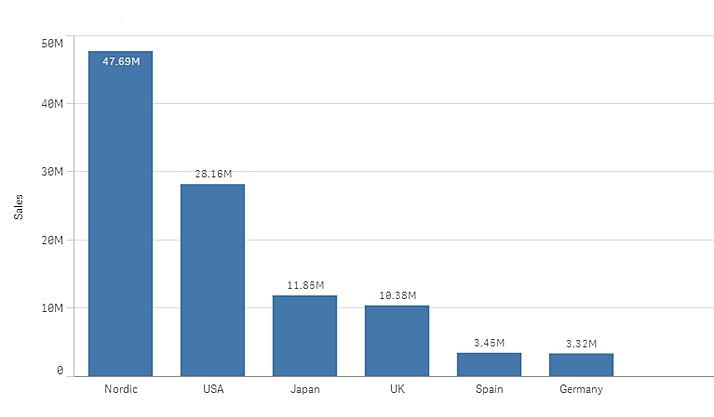
\includegraphics[width=0.25\textwidth]{grafico}
\label{fig:refejem1}
\end{figure}
 
Como puede ver en la figura \ref{fig:refejem1}, en la P.# \pageref{fig:refejem1}.
\end{lstlisting}

Las referencias una vez compiladas se ven como:
\begin{figure}[H]
    \centering
    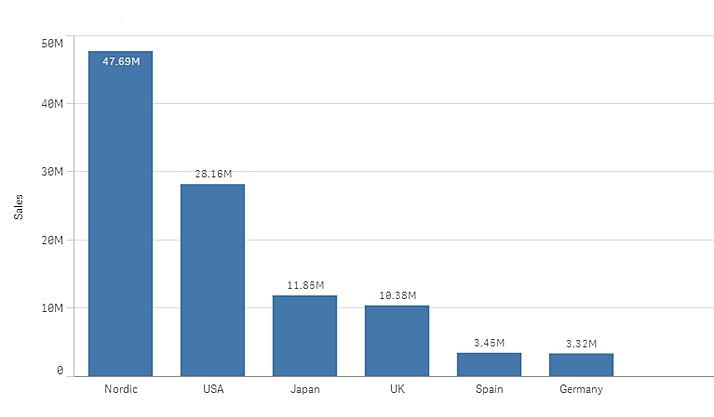
\includegraphics[width=0.25\textwidth]{grafico}
    \caption{refejem1}
    \label{fig:refejem1}
\end{figure}
 
En la figura \ref{fig:refejem1} en la P.\# \pageref{fig:refejem1}.

\section{Manejo de figuras al lado de tablas (minipage)}
El minipage es una funcionalidad de Latex utilizada para poner lado a lado estructuras que de otra forma ser\'{\i}a dif\'{\i}cil, su armaz\'{o}n en c\'{o}digo se ve como:

\begin{lstlisting}
\begin{minipage}[ajuste]{ancho del minipage}
  Texto ... \ \
  Imagenes ... \ \
  Tablas ... \ \
\end{minipage} 
\end{lstlisting}

Partiendo de esta implementaci\'{o}n se pueden crear diferentes configuraciones.

Ejemplo de tabla + tabla.

\begin{lstlisting}
\begin{minipage}{0.2\textwidth}
\begin{tabular}{|c|c|c|}
\hline
 A & B & C \\
\hline
 1 & 2 & 3  \\
\hline 
 4 & 5 & 6 \\
\hline
\end{tabular}
\end{minipage}
\begin{minipage}{0.2\textwidth}
\begin{tabular}{c|c|c}
 A & B & C \\
\hline
 1 & 2 & 3  \\
\hline 
 4 & 5 & 6 \\
\end{tabular}
\end{minipage}
\end{lstlisting}

\begin{minipage}{0.2\textwidth}
\begin{tabular}{|c|c|c|}
\hline
 A & B & C \\
\hline
 1 & 2 & 3  \\
\hline 
 4 & 5 & 6 \\
\hline
\end{tabular}
\end{minipage}
\begin{minipage}{0.2\textwidth}
\begin{tabular}{c|c|c}
 A & B & C \\
\hline
 1 & 2 & 3  \\
\hline 
 4 & 5 & 6 \\
\end{tabular}
\end{minipage}
\\
\\
Ejemplo de imagen + texto.

\begin{lstlisting}
\begin{minipage}[t]{0.2\textwidth}

\includegraphics[scale=0.4]{tec-logo}
\end{minipage}
\begin{minipage}{0.2\textwidth}
Tecnologico de CR\\
Tecnologico de CR\\
Tecnologico de CR\\
Tecnologico de CR\\
Tecnologico de CR\\
\end{minipage}
\end{lstlisting}

\begin{minipage}[t]{0.2\textwidth}

\includegraphics[scale=0.4]{tec-logo}
\end{minipage}
\begin{minipage}{0.2\textwidth}
Tecnol\'{o}gico de CR\\
Tecnol\'{o}gico de CR\\
Tecnol\'{o}gico de CR\\
Tecnol\'{o}gico de CR\\
Tecnol\'{o}gico de CR\\
\end{minipage}

Ejemplos de imagen + imagen + imagen.

\begin{lstlisting}
\begin{minipage}[b]{0.15\textwidth}

\includegraphics[width=\textwidth]{tec-logo}
\end{minipage}
\begin{minipage}[t]{0.15\textwidth}

\includegraphics[width=\textwidth]{tec-logo}
\end{minipage}
\begin{minipage}[t]{0.15\textwidth}

\includegraphics[width=\textwidth]{tec-logo}
\end{minipage}
\end{lstlisting}

\begin{minipage}[b]{0.15\textwidth}

\includegraphics[width=\textwidth]{tec-logo}
\end{minipage}
\begin{minipage}[t]{0.15\textwidth}

\includegraphics[width=\textwidth]{tec-logo}
\end{minipage}
\begin{minipage}[t]{0.15\textwidth}

\includegraphics[width=\textwidth]{tec-logo}
\end{minipage}

\section{Ecuaciones matem\'aticas}
En este segmento se presentan las caracter\'{\i}sticas b\'{a}sicas para generar f\'{o}rmulas matem\'{a}ticas en Latex.

\subsection{Modo matem\'{a}ticas}
Latex permite dos tipos de f\'{o}rmulas: inline y display, la primera permite escribir la f\'{o}rmula en l\'{\i}nea con el texto y la segunda lo opuesto, por lo que cuando se escriba ocupar\'{a} una l\'{\i}nea completa por si sola.\par
Las f\'{o}rmulas \textquotedblleft{}inline\textquotedblright{} se caracterizan por estar delimitadas por \textdollar{}formula\textdollar{} y las \textquotedblleft{}display\textquotedblright{} por \textdollar{}\textdollar{}formula\textdollar{}\textdollar{} o \textbackslash{}begin\{equation\} formula \textbackslash{}end\{equation\}. Cabe recalcar que en el modo inline las expresiones son compresas para seguir con la l\'{\i}nea del texto.

Ejemplo de inline:

\begin{lstlisting}
La formula $E=MC^2$ fue formulada por Einstein anos despues de presentar su teoria de la relativadad.
\end{lstlisting}

La f\'{o}rmula $E=MC^2$ fue formulada por Einstein a\~{n}os despu\'{e}s de presentar su teor\'{i}a de la relativadad.

Ejemplo de display:
\begin{lstlisting}
La formula $$E=MC^2$$ fue formulada por Einstein anos despues de presentar su teoria de la relativadad.En unidades naturales ($c$ = 1), representa la identidad

\begin{equation}
E = m
\end{equation}
\end{lstlisting}
La f\'{o}rmula $$E=MC^2$$ fue formulada por Einstein a\~{n}os despu\'{e}s de presentar su teor\'{i}a de la relativadad.En unidades naturales ($c$ = 1), representa la identidad

\begin{equation}
E = m
\end{equation}

\subsection{S\'{i}mbolos especiales}
La utilizaci\'{o}n de s\'{\i}mbolos especiales se da por el modo matem\'{a}tica explicado en el punto anterior, solamente basta escribir \textbackslash{}simbolo dentro de los \textdollar{} \textdollar{}.

\begin{lstlisting}
$$\delta \alpha$$
\end{lstlisting}

$$\delta \alpha$$

\subsection{Fracciones}

Las fracciones pueden ser utilizadas en conjunto con el texto $\frac{1}{2} $ o por si solas con los modos inline y display.

$$\frac{1}{2} $$

Las fracciones son muy vers\'{a}tiles, pudiendo ser anidadas para expresiones complejas.

\begin{lstlisting}
Ejemplo sencillo:

$$\frac{1}{2}$$

Ejemplo anidado:
 
$$ \frac{1+\frac{a}{b}}{1+\frac{1}{1+\frac{1}{a}}} $$
 
\end{lstlisting}

Ejemplo sencillo:

$$\frac{1}{2}$$

Ejemplo anidado:
 
$$ \frac{1+\frac{a}{b}}{1+\frac{1}{1+\frac{1}{a}}} $$
 
\subsection{Operadores}
El manejo de operadores es muy variado por lo que a continuaci\'{o}n se explican los m\'{a}s utilizados.

$$\int_{a}^{b} x^2 dx$$

Las integrales como la anterior son definidas en Latex como:

\begin{lstlisting}
\int_{superior}^{inferior}

$$\int_{a}^{b} x^2 dx$$
\end{lstlisting}

Integrales anidadas pueden resultar más complejas, pero se pueden obtener modificando el inicio de la expresión (int) como en los siguientes ejemplos:
\begin{lstlisting}
$$\iint_V \mu(u,v) \,du\,dv$$
$$\iiint_V \mu(u,v,w) \,du\,dv\,dw$$
$$\idotsint_V \mu(u_1,\dots,u_k) \,du_1 \dots du_k$$
\end{lstlisting}

$$\iint_V \mu(u,v) \,du\,dv$$
$$\iiint_V \mu(u,v,w) \,du\,dv\,dw$$
$$\idotsint_V \mu(u_1,\dots,u_k) \,du_1 \dots du_k$$

Al igual que las integrales, las sumatorias est\'{a}n dadas por:
\begin{lstlisting}
\sum_{superior}^{inferior}

Ejemplo:
Sum $\sum_{n=1}^{\infty} 2^{-n} = 1$ inside text
\end{lstlisting}

$$\sum_{n=1}^{\infty} 2^{-n} = 1$$

En el caso de los l\'{i}mites se utiliza el comando

\begin{lstlisting}
\lim_{lower}

Ejemplo:
$$\lim_{x\to\infty} f(x)$$
\end{lstlisting}

$$\lim_{x\to\infty} f(x)$$

\section{Manejo de colores}
El manejo de colores en Latex est\'{a} dado por los paquetes

\begin{lstlisting}
\usepackage{color}
\usepackage{xcolor}
\end{lstlisting}

Ambos paquetes permiten la manipulaci\'{o}n de colores, pero a la vez tiene la flexibilidad de modificar los colores y secciones a gusto. El siguiente ejemplo muestra los colores predefinidos.

\begin{lstlisting}
\begin{itemize}
\color{blue}
\item Primer item
\item Segundo item
\end{itemize}
 
\noindent
{\color{red} \rule{\linewidth}{0.5mm} }
\end{lstlisting}

\begin{itemize}
\color{blue}
\item Primer item
\item Segundo item
\end{itemize}
 
\noindent
{\color{red} \rule{\linewidth}{0.5mm} }

Los colores red y blue est\'{a} predefinidos en el paquete color, algunos otros ejemplos b\'{a}sicos son.

\begin{lstlisting}
El color del texto puede ser cambiado a \textcolor{red}{rojo}. Tambien puede cambiar el background del \colorbox{BurntOrange}{texto}.
\end{lstlisting}

El color del texto puede ser cambiado a \textcolor{red}{rojo}. Tambien puede cambiar el background del \colorbox{orange}{texto}.\par{}

Para una mayor variedad de colores se pueden crear variables de color d\'{a}ndole una etiqueta a un valor RGB.

\begin{lstlisting}
\definecolor{rosado}{rgb}{0.858, 0.188, 0.478}
\definecolor{gris}{gray}{0.6}
\end{lstlisting}

\definecolor{rosado}{rgb}{0.858, 0.188, 0.478}
\definecolor{gris}{gray}{0.6}

\begin{enumerate}
\item \textcolor{rosado}{Rosado}
\item \textcolor{gris}{Gris}
\end{enumerate}

El definecolor utiliza una de las siguientes 4 opciones para el primer par\'{a}metro.

\begin{enumerate}
\item \textbf{rgb}: rojo, verde, azul. Tres valores separados por comas entre 0 y 1 definen los componentes del color.
\item \textbf{RGB}: lo mismo que rgb, pero los n\'{u}meros son enteros entre 0 y 255.
\item \textbf{cmyk}: cian, magenta, amarillo y blacK. Lista de cuatro n\'{u}meros separados por comas entre 0 y 1 que determina el color de acuerdo con el modelo aditivo utilizado en la mayor\'{\i}a de las impresoras.
\item \textbf{gray}: escala de grises. Un solo n\'{u}mero entre 0 y 1.
\end{enumerate}

Adem\'{a} de modificar el color del texto de puede cambiar el color de la p\'{a}gina con

\begin{lstlisting}
\pagecolor{black}
\end{lstlisting}


\includegraphics[scale=1]{ejemplofondo}

\begin{thebibliography}{1}
\bibitem{[1]}The Editors of Encyclopaedia Britannica  (2013) \emph{LaTeX COMPUTER PROGRAMMING LANGUAGE} [Blog post]. Consultado desde https://www.britannica.com/technology/LaTeX-computer-programming-language
\bibitem{[2]} \emph{Introduction to LaTeX.} (2018). Consultado desde https://www.latex-project.org/about/
\bibitem{[3]} \emph{Basic description of file types and how LaTeX works.} (2018). Consultado desde http://personal.bgsu.edu/~zirbel/5920/latex/latex\_basics.htm
\bibitem{a} \emph{Latex-Tutorial.} (2018). Consultado desde https://www.latex-tutorial.com
\bibitem{b} \emph{ShareLatex.} (2018). Consultado desde https://www.sharelatex.com/learn
\bibitem{c} \emph{Sascha-Frank.} (2018). Consultado desde http://www.sascha-frank.com


\end{thebibliography}
\end{document}






